\documentclass[../SOP.tex]{subfile}

\begin{document}
% Skeln mellem kostfunktion og præcision i afsnit om kostfunktion
\section{Træning af et neuralt netværk}
Der er nu konstrueret et neuralt netværk, som kan tage et billede som input og give et resultat. Dette resultat er dog ikke brugbart endnu, da netværket ikke er blevet trænet.
\subsection{Kostfunktionen}
For at kunne træne et netværk, skal der først defineres en funktion som fortæller hvor tæt netværket er på det korrekte svar. Denne funktion kaldes \emph{kostfunktionen} eller \emph{fejlfunktionen}, og vil her defineres som:
\begin{gather}
  E_t(\mathbf{o})=\frac{1}{2}\sum_{k=1}^n(t_k-o_k)^2 \label{eq:cost}\\
  E_t\colon \R^n\rightarrow\R\nonumber
\end{gather}
Her er $\mathbf{o}$ netværkets outputs, og $\mathbf{t}$ den forventede værdi af den tilsvarende knude.\\
Denne funktion kan udvides for at bestemme fejlen for et helt datasæt:
\begin{equation}
  E(\mathbf{w})=\frac{1}{2}\sum_{t\in T}\sum_{k\in outputs}(t_{kd}-o_{kd})^2
  \label{eq:costset}
\end{equation}
Kostfunktionen er dog ikke specielt brugbar til at vurdere netværkets præstation for mennesker, da den ikke siger noget om hvor ofte netværket gætter rigtigt. Her indføres præcisionen af netværket:
\begin{equation*}
  P=\frac{c}{t}
\end{equation*}
Her er $c$ antallet af korrekte gæt netværket har lavet, og $t$ er det totale antal gæt netværket har lavet. Bemærk at denne funktion ikke direkte bruges til at træne netværket, men er blot en måde at kunne sammenligne modeller.
\subsection{Gradient nedstigning}
Eftersom netværkets præstation nu kan måles ud fra værdien af en enkelt funktion, er målet nu at få værdien af denne funktion så tæt på 0 som muligt, for alle træningseksempler. Da dette er et optimeringsproblem, vil den åbenlyse løsning være at differentiere funktionen og sætte den differentierede lig med 0. Dette er dog ikke en praktisk løsning, da denne funktion vil være meget kompleks når den udvides, idet det vil vise sig at, et netværk som skal kunne genkende relativt små billeder, vil have tusindvis af vægte, hvilket gør den upraktisk at differentiere. Løsningen som Machine Learning præsenterer er at bruge gradienten til at gradvist nærme sig et lokalt minimum. Denne algoritme kaldes \emph{gradient nedstigning}. Først bestemmes gradienten, ved partiel differentiering:
\begin{equation}
  \nabla E(\mathbf{w})=\begin{bmatrix}
    \pfrac{E}{w_0} & \pfrac{E}{w_1} & \dots & \pfrac{E}{w_n}
  \end{bmatrix}
  \label{eq:gradError}
\end{equation}
Ud fra dette kan ændringen i vægtene bestemmes som:
\begin{gather}
  \Delta \mathbf{w} = -\eta \nabla E(\mathbf{w}) \label{eq:trgrad}\\ 
  \mathbf{w} \leftarrow \mathbf{w} + \Delta\mathbf{w}
\end{gather}
Her er $\eta$ \emph{læringsraten}, som er et tal, $\eta>0$, $\eta\in\R$, som bestemmer hvor hurtigt modellen bevæger sig i retningen af den stejleste nedstigning \parencite{mitch}. Denne parameter er vigtig, da en for lav læringsrate vil resultere i at netværket nærmer sig et lokalt minimum for langsomt, mens en for høj værdi vil resultere i at netværket ``rammer forbi'' det lokale minimum \parencite{learningrate}. Eksempler på disse ses på figur \ref{fig:learningrate}.
\begin{figure}[ht]
  \centering
  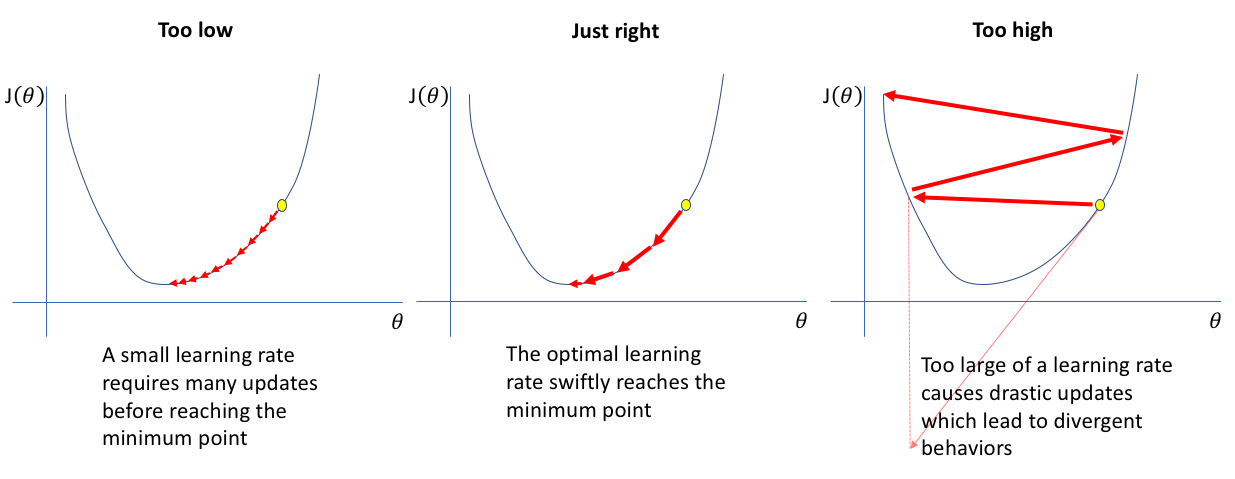
\includegraphics[width=\textwidth]{learningrate.png}
  \caption{En visualisering af læringsratens indvirkning på et neuralt netværk \parencite{learningrate}}
  \label{fig:learningrate}
\end{figure}

\subsection{Udledning af træningsreglen}
For at bestemme hvor meget hver vægt skal ændres, skal gradienten, som vist i ligning \ref{eq:gradError}, bestemmes. $\pfrac{E}{w_{jk}}$ skal derfor bestemmes. Dette gøres på to forskellige måder, afhængigt af om knude $j$ er en output knude eller en skjult knude.
\subsubsection{Outputvægte}
Først skal fejlen, som funktion af vægten bestemmes. Da vægten kun kan have indflydelse på en outputknude, kan de andre ignoreres.
\begin{equation*}
  E(w_{jk})=\frac{1}{2}(t_j-\sigma(w_{jk}o_k))^2
\end{equation*}
Her kan kædereglen bruges til at differentiere udtrykket, ved hjælp af de værdier der allerede er definerede:
\begin{equation*}
  \pfrac{E}{w_{jk}}=\pfrac{E}{o_j}\cdot\pfrac{o_j}{x_j}\cdot\pfrac{x_j}{w_{jk}}
\end{equation*}
Det sidste udtryk kan bestemmes som:
\begin{equation*}
  \pfrac{x_j}{w_{jk}}=o_k
\end{equation*}
Herfra skal $\pfrac{E}{o_j}$ bestemmes:
\begin{align*}
  \pfrac{E}{o_j}&=\pfrac{}{o_j}\frac{1}{2}(t_j-o_j)^2\\
  &= (t_j-o_j)\pfrac{}{o_j}(t_j-o_j)\\
  &= (t_j-o_j)\cdot-1\\
  &= -(t_j-o_j)
\end{align*}
Det gælder at:
\begin{equation*}
  \sigma'(x)=\sigma(x)\cdot(1-\sigma(x))
\end{equation*}
$\pfrac{o_j}{x_j}$ kan derfor bestemmes som:
\begin{equation*}
  \pfrac{o_j}{x_j}=\pfrac{\sigma(x_j)}{x_j}=o_j\cdot(1-o_j)
\end{equation*}
Alt dette kan samles til:
\begin{equation}
  \pfrac{E}{w_jk}=(t_j-o_j)\cdot o_j \cdot (1-o_j)\cdot o_k
  \label{eq:errorWeight}
\end{equation}
Dette samles med ligning \ref{eq:trgrad}:
\begin{equation}
  \Delta w_{jk}=\eta\cdot (t_j-o_j)\cdot o_j\cdot(1-o_j)\cdot o_k
  \label{eq:trOutput}
\end{equation}
Ud fra dette indføres en ny variabel, $\delta_j$:
\begin{equation}
  \delta_j =-\pfrac{E}{x_j}=o_j\cdot(1-o_j)\cdot(t_j-o_j)
  \label{eq:delta}
\end{equation}

\subsubsection{Skjulte vægte}
Ændringen af vægten i skjulte knuder er lidt mere indviklet, da hver vægt kan have indvirkning på mere end en outputknude. Her vil det være brugbart at referere til alle knuder, hvis værdi direkte afhænger af værdien af knude $j$. Her indføres $Ds(j)$. Kædereglen bruges igen til at finde $\pfrac{E}{w_{jk}}$. Her vil det dog også gælde at:
\begin{equation*}
  \pfrac{x_j}{w_{jk}}=o_k
\end{equation*}
Hvilket kan genbruges senere.\\

Der skal nu bestemmes $\pfrac{E}{x_j}$:
\begin{align*}
  \pfrac{E}{x_j}&=\sum_{k\in Ds(j)} \pfrac{E}{x_k}\cdot \pfrac{x_k}{x_j}\\
  \intertext{$\delta_k$ kan nu indføres, jf. ligning \ref{eq:delta}}
  \pfrac{E}{x_j}&=\sum_{k\in Ds(j)} -\delta_k\cdot \pfrac{x_k}{x_j}\\
  &= \sum_{k\in Ds(j)} -\delta_k \cdot \pfrac{x_k}{o_j}\cdot\pfrac{o_j}{x_j}\\
  &= \sum_{k\in Ds(j)} -\delta_k \cdot w_{kj}\cdot \pfrac{o_j}{x_j}\\
  &= \sum_{k\in Ds(j)} -\delta_k \cdot w_{kj}\cdot o_j\cdot(1-o_j)\\
  &= o_j\cdot(1-o_j)\sum_{k\in Ds(j)} -\delta_k \cdot w_{kj}
\end{align*}
Dette opskrives som $\delta_j=-\pfrac{E}{x_j}$:
\begin{equation}
  \delta_j=o_j\cdot(1-o_j)\cdot\sum_{k\in Ds(j)} \delta_k\cdot w_{kj} 
  \label{eq:delta_h}
\end{equation}
Jf. ligning \ref{eq:trgrad}, vil ændringen af vægten $w_{jk}$ være:
\begin{equation}
  \Delta w_{jk}=\eta\cdot \delta_j\cdot o_{k}
  \label{eq:wchange}
\end{equation}

\subsection{Backpropogation}
\begin{minipage}{\textwidth}
  Der kan nu beskrives en algoritme for hvordan et neuralt netværk trænes \parencite{mitch}:\\
  For hvert træningseksempel, med input $\mathbf{x}$ og forventede værdi $\mathbf{t}$:\\
  \textbf{Feed-forward:}
  \begin{enumerate}
    \item Sæt værdien af inputlaget af netværket til $\mathbf{x}$
    \item Bestem outputværdien for hver knude i alle lag, indtil alle værdier af outputknuderne er bestemte.
  \end{enumerate}
  \textbf{Backpropogation:}
  \begin{enumerate}[resume]
    \item For hver outputknude $k$, bestem $\delta_k$ (Se ligning \ref{eq:delta}):
      \begin{equation*}
        \delta_k = o_k\cdot (1-o_k)\cdot(t_k-o_k)
      \end{equation*}
    \item For hver skjulte knude, bestem $\delta_h$ (Se ligning \ref{eq:delta_h}):
      \begin{equation*}
        \delta_h = o_h\cdot(1-o_h) \sum_{k\in Ds(h)} w_{kh}\delta_k
      \end{equation*}
    \item Beregn ændringen for hver vægt (Se ligning \ref{eq:wchange}):
      \begin{equation*}
        \Delta w_{jk} = \eta\cdot\delta_j\cdot o_k
      \end{equation*}
    \item Opdater hver vægt:
      \begin{equation*}
        w_{jk} \leftarrow \Delta w_{jk} + w_{jk}
      \end{equation*}
  \end{enumerate}
\end{minipage}
Denne specifikke algoritme kaldes \emph{stokastisk gradient nedstigning}. I modsætning til almindelig gradient nedstigning, justeres vægtene efter hvert træningseksempel, hvilket gør træningen markant hurtigere.

\end{document}
